

\tikzset{every picture/.style={line width=0.75pt}} %set default line width to 0.75pt        

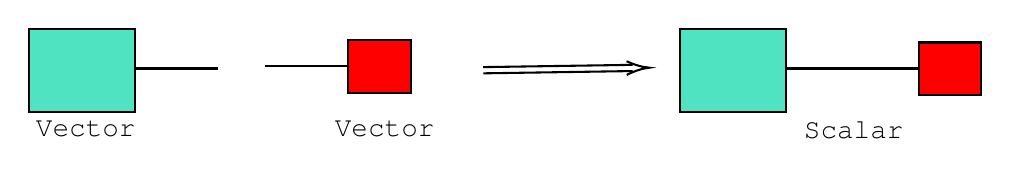
\begin{tikzpicture}[x=0.75pt,y=0.75pt,yscale=-1,xscale=1]
%uncomment if require: \path (0,300); %set diagram left start at 0, and has height of 300

%Shape: Rectangle [id:dp5798300081474196] 
\draw  [fill={rgb, 255:red, 80; green, 227; blue, 194 }  ,fill opacity=1 ] (100,112) -- (151,112) -- (151,152) -- (100,152) -- cycle ;
%Straight Lines [id:da22962560201461135] 
\draw [fill={rgb, 255:red, 80; green, 227; blue, 194 }  ,fill opacity=1 ]   (151,131.18) -- (191,131.18) ;
%Shape: Rectangle [id:dp20432070859726514] 
\draw  [fill={rgb, 255:red, 255; green, 0; blue, 0 }  ,fill opacity=1 ] (254,117.63) -- (284,117.63) -- (284,143) -- (254,143) -- cycle ;
%Straight Lines [id:da524122200138993] 
\draw [fill={rgb, 255:red, 255; green, 0; blue, 0 }  ,fill opacity=1 ]   (214,130.18) -- (254,130.18) ;

%Straight Lines [id:da7051909181445478] 
\draw    (318.98,130.5) -- (390.98,129.41)(319.02,133.5) -- (391.02,132.4) ;
\draw [shift={(399,130.78)}, rotate = 179.13] [color={rgb, 255:red, 0; green, 0; blue, 0 }  ][line width=0.75]    (10.93,-3.29) .. controls (6.95,-1.4) and (3.31,-0.3) .. (0,0) .. controls (3.31,0.3) and (6.95,1.4) .. (10.93,3.29)   ;
%Shape: Rectangle [id:dp6270655055347218] 
\draw  [fill={rgb, 255:red, 80; green, 227; blue, 194 }  ,fill opacity=1 ] (414,112) -- (465,112) -- (465,152) -- (414,152) -- cycle ;
%Straight Lines [id:da6216765005210074] 
\draw [fill={rgb, 255:red, 80; green, 227; blue, 194 }  ,fill opacity=1 ]   (465,131.18) -- (505,131.18) ;
%Shape: Rectangle [id:dp601921472040452] 
\draw  [fill={rgb, 255:red, 255; green, 0; blue, 0 }  ,fill opacity=1 ] (529,118.63) -- (559,118.63) -- (559,144) -- (529,144) -- cycle ;
%Straight Lines [id:da020089358658374357] 
\draw [fill={rgb, 255:red, 255; green, 0; blue, 0 }  ,fill opacity=1 ]   (489,131.18) -- (529,131.18) ;


% Text Node
\draw (102,155) node [anchor=north west][inner sep=0.75pt]   [align=left] {{\fontfamily{pcr}\selectfont Vector}};
% Text Node
\draw (246,155) node [anchor=north west][inner sep=0.75pt]   [align=left] {{\fontfamily{pcr}\selectfont Vector}};
% Text Node
\draw (472,155) node [anchor=north west][inner sep=0.75pt]   [align=left] {{\fontfamily{pcr}\selectfont Scalar}};


\end{tikzpicture}
